
\begin{figure}[p]
    \centering
    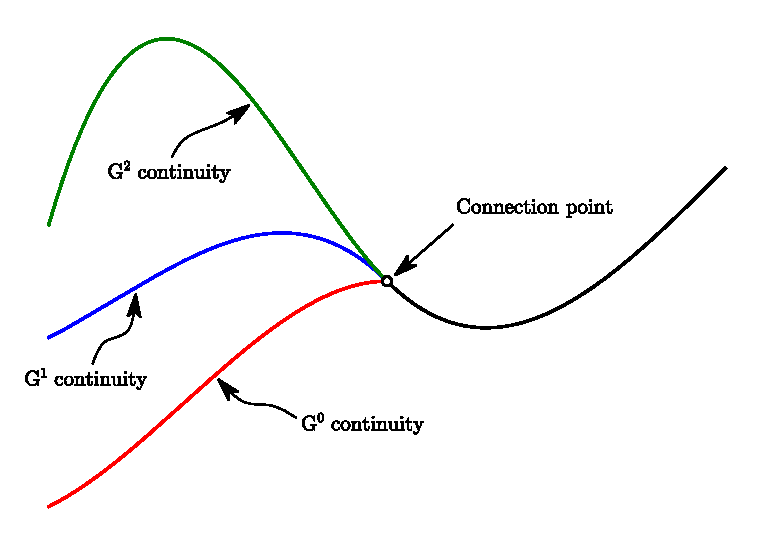
\includegraphics[width=0.8\linewidth]{1figures/curve_smoothness_annotated.pdf}
    \caption{Geometric continuity at the connection point between two curve segments}
    \label{fig:curve_smoothness}
\end{figure}

\begin{figure}[p]
    \centering
    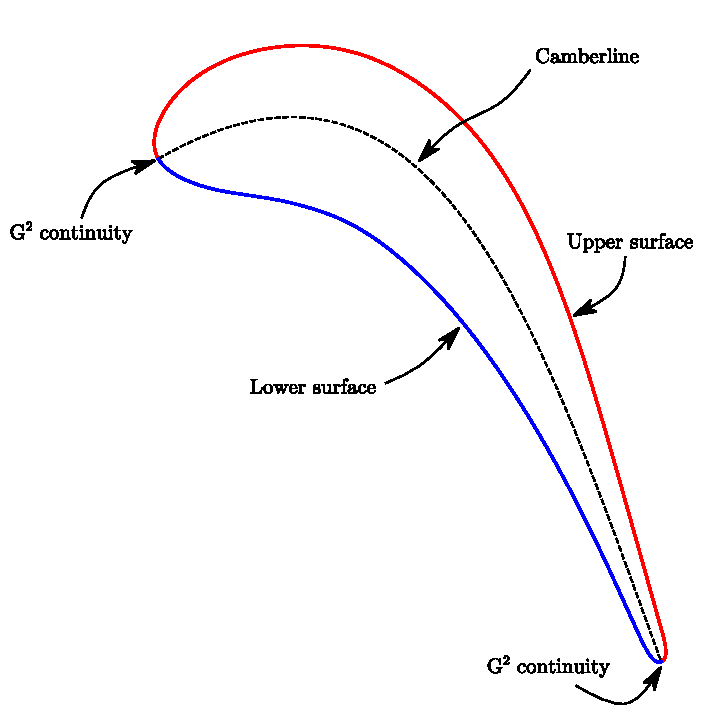
\includegraphics[width=0.8\linewidth]{1figures/G2_continutity_blade_annotated.pdf}
    \caption{G$^2$ continuity at the points connecting the upper and lower surfaces of and airfoil}
    \label{fig:G2_continutity_blade}
\end{figure}

\begin{figure}[p]
    \centering
    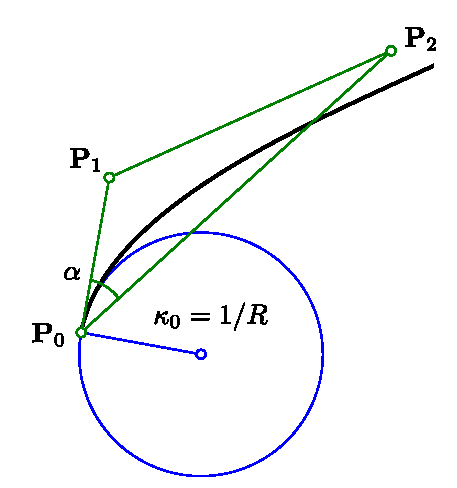
\includegraphics[width=0.5\linewidth]{1figures/endpoint_curvature_annotated.pdf}
    \caption{Curvature of a \Bezier or B-Spline curve at the endpoint $u=0$}
    \label{fig:endpoint_curvature}
\end{figure}

\begin{figure}[p]
    \centering
    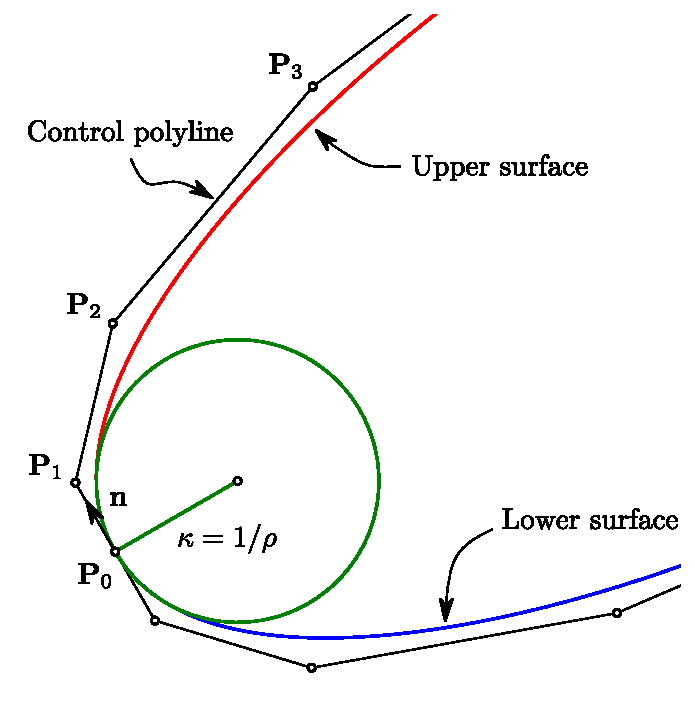
\includegraphics[width=0.65\linewidth]{1figures/leading_edge_construction_annotated.pdf}
    \caption{Construction of the leading edge of an airfoil ensuring G$^2$ continuity}
    \label{fig:leading_edge_construction}
\end{figure}
